\documentclass[12pt]{article}
\usepackage{amsmath,amssymb,parskip,custom,graphicx}
\usepackage[margin=1in]{geometry}

\begin{document}

\title{ECE 140 - Linear Circuits}
\author{Kevin Carruthers}
\date{\vspace{-2ex}Fall 2012}
\maketitle\HRule

\section*{Basic Components and Electric Circuits}
\subsection*{Units and Scales}
The international standard is {\bf SI units}. Under this system, electric current is measured in Amperes (A), work and energy is measured in Joules (J), and power, or the rate in which work is done, is measured in Watts (W).

In increasing order, from $10^{-18}$ and ascending in factors of three, the prefixes we use are atto, femto, pico, nano, micro, milli, kilo, Mega, Giga, and tera.

\subsection*{Charge, Current, Voltage, and Power}
\subsubsection*{Charge}
The basic unit of positive {\bf charge} is the proton. The unit of negative charge is the electron. We can neither create nor destroy charges.

{\bf Electric current} is defined as charge in motion, and follows the direction of the flow of positive charge (opposite the direction of electron flow). The fundamental unit of charge is the Coulomb (C).

A proton or electron has a charge of $\pm 1.602 * 10^{-19}$

\subsubsection*{Current}
Moving charges create an {\bf electrical current}. In moving charges from one place to another, we may also transfer energy. By changing the current (with respect to time), we can transfer information. Current, then, is the rate at which the charges are moving past a given reference point in a specific direction.

The charge transfered between times $t_0$ and $t_1$ can be expressed as \[ \dint{t_0}{t_1}{}{q(\tau)} = \dint{t_0}{t_1}{i(\tau)}{\tau} \] and the total charge transfered is given by \[ q(t_1) = q(t_0) + \dint{t_0}{t_1}{i(\tau)}{\tau} \]

\subsubsection*{Voltage}
Let a general 2-terminal circuit element have two terminals (ie. resistors, inductors, batteries...). There are thus two paths by which the current may enter or leave the element. If you want to push charges through a circuit element, you have to expend some energy. The energy used to push charge through an element is defined as the {\bf voltage} between the two terminals, or the potential difference.

In other words, the {\bf voltage} across a terminal pair is a measure of the work required to move charge through that element.

Voltage is measured in Volts (V), where \[ 1V = \frac{1J}{1C} \]

A voltage can exist between a pair of terminals whether or not a current is flowing. According to the Conservation of Energy, the energy expended in forcing charge through an element must appear elsewhere (ie. transformed into heat energy).

Energy could be supplied to an element or by an element.

\subsubsection*{Power}
Power is defined as the rate at which work is done or energy is expended. It is measured in Watts (W), where \[ 1W = \frac{1J}{1s} \]

If one Joule of energy is expended in transfering one Coulomb of energy through a device in one second, then we have $1W = \frac{1J}{1s} = \frac{1J}{1C}*\frac{1C}{1s}$

As such, we have \[ P = VI \]

If we have current entering the positive terminal of an element (ie. the terminal with a larger voltage), we follow the {\bf passive sign convention}. As such, the power absorbed by the element is $vi$ and the power generated or supplied by the element is $-vi$.

\subsection*{Voltage and Current Sources}
The mathematical models used for circuit analysis are only approximations. They depend on the relation between voltage across their terminals and the current going through them.

\begin{table}[ht]
\centering
  \begin{tabular}{clc}
  Relationship Between $v$ and $i$ & Element \\ \hline
  $v \propto i$ & Resistor \\
  $v \propto \fracd{i}{t}$ & Inductor \\
  $v \propto \inint{i(t)}{t}$ & Capacitor \\
  $v \not\propto i$ & Independant Voltage Source \\
  $i \not\propto v$ & Independant Current Source \\
  $v$ or $i \propto v_0$ or $i_0$ & Dependant Source \\ \hline
  \end{tabular}
\end{table}

\subsubsection*{Independant Voltage Sources}
The voltage of an {\bf independant voltage source} is completely independant of the current. It is ideal because it does not exactly represent any real physical device, but it is a reasonable approximation of some. For example, household electrical outlets can be approximated as independant voltage sources providing $115\sqrt{2}\cos(120\pi *t)$ volts. This approximation is valid for currents less than 20 A.

If the terminal voltage is constant, we have a DC voltage source. Otherwise (ie. it provides a sinusoidal output) our source is AC.

It is denoted by a circular shape with plus and minus symbols denoting the difference in voltage. An optional tilde denotes AC voltage.

\subsubsection*{Independant Current Sources}
The current of an {\bf independant current source} is completely independant of the voltage across the source. If it provides constant current, we have a DC source, otherwise it is an AC source.

Voltage across a current source is not known, it depends on the circuit connected to it.

It is denoted by a circular shape with an arrow in the direction of current flow. An optional tilde denotes AC current.

\subsubsection*{Dependant Sources, aka Controlled Sources}
A {\bf dependant source} is one where the source quantity of either voltage or current is determined by a voltage or current elsewhere in the circuit. They usually appear in equivalent electrical models for devices such as operational amplifiers or transistors.

It is denoted by a diamond shape.

\subsection*{Networks and Circuits}
An {\bf electrical network} is the interconnection of two or more simple circuit elements. An {\bf electrical circuit} is a network which contains at least one closed path. As such, every circuit is a network, but not all networks are circuits.

An {\bf active network} is one which contains at least one active element (ie. independant source). Alternatively, we have passive networks.

\subsection*{Resistance}
\subsubsection*{Ohm's Law}
{\bf Ohm's Law} describes the relationship between th voltage across a resistor and the current passing through it as \[ v = iR \] where resistance is measured in Ohms ($\Omega$) and $1\Omega = \frac{1V}{1A}$

Note that a linear resistor is an idealized circuit element. Actual resistors only act like linear resistors within certain ranges of current, voltage, or power, and also depend on temperature and other environmental factors.

\subsubsection*{Power Absorbtion}
Assuming we are following the passive sign convention, we have \[ P =vi = i^2R = \frac{v^2}{R} \] is the {\bf power absorbed} by a resistor. Note that resistors dissipate energy in the form of heat and/or light as they cannot store or generate it.

For a complete circuit, the absorbed power is equal to the generated power, as per conservation of energy.

\subsubsection*{Resistance of Wires}
Each material has a property called {\bf resistivity} ($\rho$) which is the measure of how "easily" electrons can travel through that material. The units of resistivity are $\Omega *m$, thus we have \[ R = \rho\frac{l}{A} \]

Usually, the resistance of wires can be approximated as $0 \Omega$

\subsubsection*{Conductance}
The {\bf conductance} is the inverse of the resistance, or \[ G = \frac{1}{R} \]

\subsection*{Short or Open Circuits}
{\bf Short circuits} are ones where $R = 0\Omega$ thus $V = 0V$ for any $i$. {\bf Open circuits} are ones where $R = \infty\Omega$ thus $i = 0A$ for any $v$. We will assume wires to be a perfect short circuit.

\section*{Voltage and Current Laws}
\subsection*{Nodes, Paths, Loops, and Branches}
A {\bf node} is a point at which two or more elements in a circuit have a common connection. Since we assume all wires are perfectly conducting, any wire attached to a node is considered part of a node.

Note that each element has a node at each end.

A {\bf path} is a route through a circuit where no node is encountered more than once. If we end at the same node as we started at, we have a {\bf path}. A {\bf branch} is a single path in a network composed of one simple element and the nodes at each end of that element.

\subsection*{Kirchoff's Current Law (KCL)}
\theorem{Theorem: The algebraic sum of all currents entering any node is zero.}

KCL is based on the principle of conservation of charge. Basically, charge can not accumulate at a node, so any charge entering a node must leave it. Consider an intersection: the number of cars entering an intersection is exactly equal to the number of cars leaving that intersection.

KCL can also be written as "the sum of the currents entering a node is equal to the sum of currents leaving a node".

\subsection*{Kirchoff's Voltage Law (KVL)}
\theorem{Theorem: The algebraic sum of the voltage around any closed path is zero.}

This is based on the fact that the enrgy required to move a charge from point A to point B must have the same value independant of the path between points.

\section*{Series and Parallel Connections}
\subsection*{Components in Series}
Circuit components that carry the same current are said to be in {\bf series}. Note that they must have the same current, not just equal currents.

\subsection*{Components in Parallel}
Circuit components are said to be in {\bf parallel} if they are connected between the same pair of nodes. Components in parallel have the same voltage drop (again, not just equal voltage drops, but the same voltage drop).

\subsection*{Connected Sources}
Several voltage sources in series may be replaced by an equivalent voltage source having a voltage equal to the algebraic sum of the individual sources. Parallel current sources may be combined by algebraicly adding the individual currents.

Ideal voltage sources in parallel are permissible only when each has the same terminal voltage at every instant. Ideal current sources in series are permissible only when each has the same current (including sign) at every instant.

\subsection*{Resistors in Series and Parallel}
We combine any number of {\bf resistors in series} by finding the algebraic sum of their resistances and replacing them with an equivelent resistor such that \[ R_{{\rm eq}} = R_0 + R_1 + \dots + R_n \]

For {\bf resistors in parallel}, we use \[ R_{{\rm eq}} = \bigl(R_0^{-1} + R_1^{-1} + \dots + R_n^{-1}\bigl)^{-1} \] and the notation \[ R_{{\rm eq}} = R_0//R_1//\dots//R_n \]

Note that we have the special case $R_0//R_1$ where $R_{{\rm eq}} = \frac{R_0R_1}{R_0 + R_1}$

\subsection*{Voltage and Current Division}
{\bf Voltage division} is used with resistors in series. To solve for the voltage across a single resistor when we have the voltage across all of them and their individual resistances, we have \[ v_k = v\frac{R_k}{R_0 + R_1 + \dots + R_k + \dots + R_n} \]

{\bf Current division} is used with resistors in parallel. If we have the network current and the resistances of each resistor, we can solve for the current across any one resistor with \[ i_k = i\frac{R_0//R_1//\dots//R_k//\dots//R_n}{R_k} \]

\section*{Ground}
In electrical circuits, we usually select a node in the circuit to be a {\bf ground}. A ground is a node having a potential of zero volts. This allows use to reference all other voltages in a circuit to the ground.

\section*{Nodal Analysis}
{\bf nodal analysis} is a methodical circuit analysis technique based on KCL. An N node circuit will have N-1 unknown voltages, and thus will need N-1 equations, where each equations is a simple KCL equation.

To perform nodal analysis, select one node to be a reference node, which will be the negative terminal of the voltages in the circuit. This reference node will be connected to ground and considered to have zero voltage. Usually, the reference node is the node with the greatest number of branches. Then, solve the system of equations formed by the KCL equations of each remaining node, with respect to the reference node.

\subsection*{Supernodes}
A {\bf supernode} is two nodes separated by an independant voltage source. In nodal analysis, we can treat this as a single node.

\section*{Mesh Analysis}
{\bf Mesh analysis} is a methodical circuit analysis technique based on KVL. It can only be applied to planar circuits.

Note: a {\bf planar circuit} is a circuit for which it is possible to draw the circuit diagram on a plane surface in such a way that no branch passes over or under anyother branch.

A {\bf mesh} is a loop which does not contain any other loops within it.

To perform mesh analysis, assign a unique {\bf mesh current} (current that flows only around the perimeter of a mesh) to each mesh, and write the KVL equation for each mesh, using the mesh currents. Solving this system of equations will solve the circuit.

If we have M meshes, we will have M Mesh currents and will write M KVL equations.

The convention is to make all mesh currents clock-wise, but you can select any arbitrary direction.

\subsection*{Supermeshes}
A {\bf supermesh} is created from two meshes that have an independant current source as a common element. In mesh analysis, we can ignore the branch containing the current source and calculate the KVL for the resulting mesh.

Note that if the current source lies on the perimeter of the circuit, there is no need to write KVL in for this mesh.

\section*{Linearity and Superposition}
\theorem{The superposition principle: The response (a desired current or voltage) in a linear circuit having more than one independant source can be obtained by adding the responses caused by the separate independant sources acting alone.}

The {\bf superposition principle} can be applied to linear circuits only.

\section*{Linear Elements}
A {\bf linear element} is one which has a linear voltage-current relationship. A linear voltage-current relationship means that if we multiply the current through an element by a constant k, this results in multiplying the voltage across the component by the same constant k.

\subsection*{Linear Circuits}
A {\bf linear circuit} is one composed entierly from independant sources, linear dependant sources, and linear elements. For any linear circuit, if all independant voltage and current sources are multiplied by a constant k, all the current and voltage responses in the circuit will be multiplied by the same factor k.

\section*{The Principle of Superposition}
If we have two inputs (independant sources), which are also referred to as "forcing functions", and two responses (or "response functions"), then when the inputs change, the responses will change.

\theorem{Theorem: In any linear resistive network, the voltage across or the current through any resistor or source can be calculated by algebraically adding all the individual voltages or currents caused by the "seperate" independat sources acting along, with all other independent sources deactivated.}

To deactivate an independant voltage source, you make it into a short circuit where $v = 0$ (replace it with a wire). To deactivate an independant current source, you make it into an open circuit where $i = 0$ (remove that branch from the circuit).

Dependant sources are left active at all times.

For any linear resistive circuit with N independant sources, we must solve the circuit N times, each time considering only one independant source and deactivating all others.

Note that if we have three independant sources, we can either consider only one source at a time, three times, or consider two sources at a time, three times. This applies to any N independant source case.

A good way to think of superposition is as follows: each source has a contribution to your result, and that contribution does not depend on the contribution of any other sources.

\section*{Source Transformation}
\subsection*{Practical Voltage Sources}
An ideal voltage source was defined as a device whose terminal voltage is independant of the current through it. An ideal voltage source can provide an unlimited amount of power, and does not practically exist.

A better approximation of a {\bf practical voltage source} is an ideal voltage source in series with a resistor. This causes the voltage to be reduced when large currents are drawn from it.

This allows us to use a combination of ideal circuit elements to model a real device. Note that any eral device is characterized by a certain current-voltage relationship at its terminals, thus we can try to develop some combination of ideal elements that can furnish a smiliar current-voltage characteristic.

For any practical voltage source, as the current increases, the voltage approaches zero, eventually reaching zero at some maximum current. The voltage when the current is zero is equal to the voltage provided by the ideal voltage source.

Note that the resistor is not "really" present as a separate component, but is only a part of the model we use to represent a practical voltage source in which the terminal voltage decreases as the load current increases.

\subsection*{Practical Current Source}
Ideal current sources can deliver a constant current regardless of the load resistance connected to it or the voltage across its terminals. Such a device does not exist in the real world.

A {\bf practical current source} is defined as an ideal current source in parallel with a resistor. As voltage across these elements increase, the current it provides decreases.

\subsection*{Equivalent Practical Sources}
Two sources are said to be {\bf equivalent} if they produce identical voltage and curretns when they are connected to identical resistances.

Identical sources provide the same open-circuit voltage and short-circuit current, though they provide different amounts of power. In essence, they are equivalent only with respect to what appears at the load terminals, but thay are not equivalent internally.

The goal of source transformation tends to be to end up with either all current sources or all voltage sources.

To perform source transformation on a voltage source in series with a resistor, replace that network with a current source in parallel with a resistor. The resistor will have the same resistance, and the current source will have a current equal to the voltage of the original source divided by the resistance of the resistor.

To perform source transformation on a current source in parallel with a resistor, replace that network with a voltage source in series with a resistor. The resistor will have the same resistance, and the voltage source will have a voltage equal to the current of the original source times the resistance of the resistor.

\section*{Thevenin's Equivalent Circuits}
\theorem{Thevenin's Theroem: It is possible to replace any linear circuit with an independant voltage source in series with a resistor.}

The response measured at the load resistor will remain unchanged, thus the original circuit and the equivalent circuit will be equivalent, from an electrical point of view.

To use Thevenin's Theorem:
\begin{enumerate}
\item Given any linear circuit, rearrange it in the form of two networks, connected by two wires. The network on the left will be made into an equivalent circuit. Ensure that the two parts of any dependant source are in the same network.
\item Disconnect the networks at the wire connections.
\item Find the open circuit voltage $V_{{\rm th}}$ across the broken wire connections (nodes).
\item To find the equivalent resistance $R_{{\rm th}}$ (chose one method)
\begin{enumerate}
\item For networks with only independant sources
\begin{itemize}
\item Deactivate any independant sources.
\item Find $R_{{\rm th}}$ between the two nodes.
\end{itemize}
\item For networks with dependant and/or independant sources, or networks without independant sources.
\begin{itemize}
\item Deactivate any independant sources.
\item Leave any dependant sources untouched.
\item Put a test voltage between the nodes and find the current across the nodes, or put a test current source and find the voltage across. Then $R_{{\rm th}} = \frac{V_t}{I_t}$
\end{itemize}
\item For networks with dependant and/or independant sources
\begin{itemize}
\item Leave all sources untouched.
\item Find the short circuit current, assuming the nodes are attached. Then $R_{{\rm th}} = \frac{V_{{\rm th}}}{I_{{\rm sc}}}$
\end{itemize}
\end{enumerate}
\end{enumerate}

\section*{Norton's Theorem}
\theorem{Norton's Theorem: It is possible to replace any circuit with an independant current source in parallel with a resistor.}

Norton's method follows in the same way as Thevenin's. Note the two equivalent circuits are related through source transformation.

\section*{Maximum Power Transfer}
\theorem{Theorem: An independant voltage source with resistance $R_S$  or an independant current source with resistance $R_S$ delivers a maximum power to the load resistance $R_L$ for which $R_S = R_L$}

Note that $R_S$ is equal to the Thevenin or Norton equivalent resistance.

Thus we have \[ P_{{\rm max}} = \frac{v^2}{4R^2} \]

\section*{Operational Amplifiers}
{\bf "Op amps"} are very useful every day electrical devices built on integrated circuits (IC). One IC may contain several op amps, and each op amp is built using many transistors.

\begin{figure}[ht]
\centering
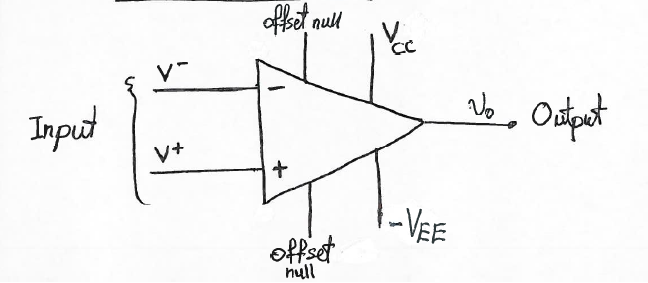
\includegraphics[width=0.8\textwidth]{opamp.png}
\end{figure}

where we have $v_{CC}$ is the positive power supply terminal, $-v_{EE}$ is the negative power supply terminal (or ground), $v^+$ is the non-inverting input, $v^-$ is the inverting input, $v_O$ is the output, and the offset null terminals are used for external adjustment to balance the op amp.

For analysis, the inner circuitry of the om amp makes no difference, and we are concerned only with the relationship between input and output.

\subsection*{Ideal Op Amps}
In practice, most op amps perform so well that we can assume we are dealing with an {\bf ideal om amp}.

Characteristics of an ideal op amp
\begin{itemize}
\item No current can enter either input terminal
\item $v_o = A_o(v^+ - v^-)$ where $A_o$ is the open loop gain and $A_o = \infty$ for ideal op amps.
\item The output terminal acts as an ideal voltage source (ie. does not vary depending on connected load).
\item $-v_{EE} \leq v_o \leq v_{CC}$
\end{itemize}

Note that if $v^+ > v^-$ then $v_o = v_{CC}$ and if $v^+ < v^-$ then $v_o = -v_{EE}$. The only way $v_o$ can be a finite number is if $-v_{EE} = v_{CC}$

In this course, we'll focus on negative feedback systems.

\begin{figure}[ht]
\centering
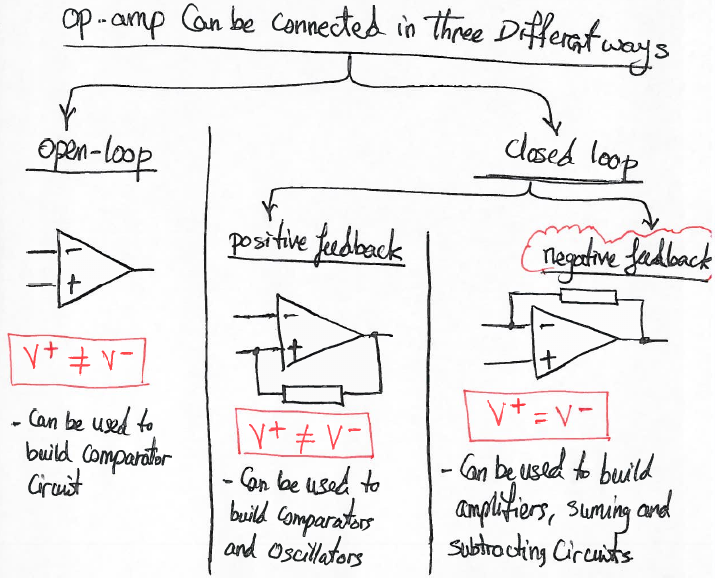
\includegraphics[width=0.8\textwidth]{opampforms.png}
\end{figure}

\subsection*{Inverting Amplifiers}

\begin{figure}[ht]
\centering
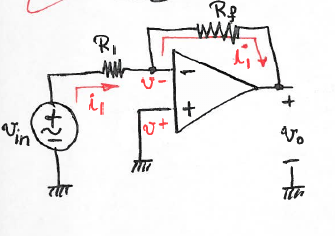
\includegraphics[width=0.5\textwidth]{invertingamp.png}
\end{figure}

Since we have negative feedback and $v^+$ is connected to the ground, $v^-$ becomes a virtual ground.

This allows us to solve this circuit by following the current, which follows a linear path. The general form of this circuit gives us \[ v_o = -\frac{R_f}{R_1}v_{{\rm in}} \]

Note that the relationship between $R_f$ and $R_1$ determines whether the om amp amplifies or attenuates the input voltage. The negative sign in the output equation means that the output and input signals are out of phase (ie there is a 180$^\circ$ phase shift between the two), thus they are {\bf inverted}.

Note that the voltage gain $A_v$ of any amplifier is equal to $\frac{v_o}{v_{{\rm in}}}$

\subsection*{Non-Inverting Amplifiers}

\begin{figure}[ht]
\centering
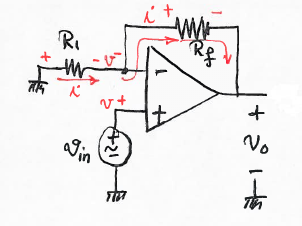
\includegraphics[width=0.5\textwidth]{noninvertingamp.png}
\end{figure}

The general form of the equation for a non-inverting amplifier is \[ v_o = v_{{\rm in}} \bigl(1 + \frac{R_f}{R_1}\bigl) \]

Note that in this case, the input and output voltages are in phase.

\subsection*{Buffers}
Note that some forms of op amps can have $v_o = v_{{\rm in}}$. This can be useful as no current is drawn from the input source, thus the om amp acts as a buffer between the input and the resistive load.

Also note that this type of op amp circuit can render some resistances inapplicable to the analysis (if no current enters it/them).

\subsection*{Summing Amplifiers}

\begin{figure}[ht]
\centering
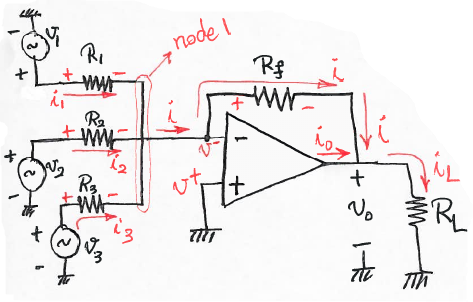
\includegraphics[width=0.7\textwidth]{summingamp.png}
\end{figure}

The general form ofthe equation for a summing amplifier is \[ v_o = -\bigg(\frac{R_f}{R_1}v_1 + \frac{R_f}{R_2}v_2 + \frac{R_f}{R_3}v_3\bigg) \]

\subsection*{Difference Amplifier}

\begin{figure}[ht]
\centering
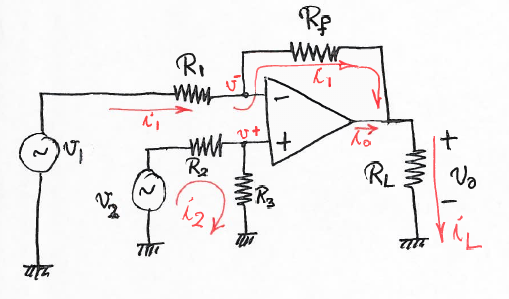
\includegraphics[width=0.7\textwidth]{differenceamp.png}
\end{figure}

This is a special-case amplifier which must be solved for each possibility. For this example circuit, the general equation is \[ v_o = \bigl(1 + \frac{R_f}{R_1}\bigl)\bigl(\frac{R_3}{R_2+R_3}\bigl)v_2 - \frac{R_f}{R_1}v_1 \]

\subsection*{Cascaded Stages}
Op amps can be {\bf cascaded} to meet certain requirements. To solve cascaded circuits, simply solve for each op amps output voltage, and then treat that as an ideal independant voltage source input for the next op amp.

\section*{Capacitors and Inductors}
{\bf Capacitors} and {\bf inductors} are passive circuit elements which can store and deliver finite amounts of energy. They differ from ideal sources in that they can not sustain a finite average power flow over an infinite time interval. Note that their voltage-current relationship is time-dependant.

\subsection*{Ideal Capacitor Model}
\textit{Active Element: an element that is capable of supplying an average power greater than zero to some external device, where the average is taken over an infinte time interval.}

\textit{Passive Element: an element that can not supply non-zero average power over an infinite time interval.}

Examples of passive elements
\begin{itemize}
\item Resistors $\to$ received energy is usually transformed into heat, and resistors cannot supply energy
\item Capacitors $\to$ received energy is stored in the form of an electric field, and this stored energy can be retrieved
\item Inductors $\to$ received energy is stored int the form of a magnetic field, and this stored energy can be retrieved
\end{itemize}

For an {\bf ideal capactitor} \[ i(t) = C\ \fracd{v(t)}{t} \] where $C$ is the capacitance, measured in farads $F$ where $1F = \frac{1C}{1V}$

If the current entering the capacitor is DC, then current flow will eventualy stop when the capacitor has accumulated enough charge. If the current is time-varying, a displacement current will flow between the plates (see unified electromagnetic theory), and the current will be non-zero.

A capacitor is denoted by two straight lines perpendicular to a wire, with empty space between them. If one of the lines is curved, it is the negative terminal.

To solve for the capacitance between two nearby plates, we have \[ C = \frac{\varepsilon A}{d} \] where $A$ is the area of the conducting surfaces, $d$ is the seperation between plates, and $\varepsilon$ is the permativity of the insulating material in farads per metre. For air or a vaccuum, $\varepsilon = 8.854 \frac{pF}{m}$

Important properties of a capactior
\begin{itemize}
\item If $v(t)$ is constant (ie DC), $i(t) = 0$, or more generally: capacitors act as open circuits for DC current
\item The voltage across the capacitor $v(t)$ cannot change suddenly (it would require infinite current to do so)
\item Only a finite amount of energy can be stored; energy is not dissipated, only stored
\end{itemize}

\subsubsection*{Integral Voltage-Current Relationships}
For $i(t) = C\ \fracd{v(t)}{t}$, we can find \[ v(t) = \frac{1}{C} \dint{t_0}{t}{i(\tau)}{\tau} + v(t_0) \] which can be written as an indefinite integral plus a constant of integration \[ v(t) = \frac{1}{C} \inint{i(t)}{t} + k \]

Usually, we have $v(-\infty) = 0$, so $v(t) = \frac{1}{C} \dint{-\infty}{t}{i(\tau)}{\tau}$

Since the integration of the current over any time interval is the charge accumulated in that period on the capacitor plate into which the current is flowing, we have \[ q(t) = Cv(t) \]

\subsubsection*{Energy Storage}
The power delivered to a capacitor is \[ P = v(t)\ C\ \fracd{v(t)}{t} \] and thus the change in {\bf energy stored} in its electric field between time instants $t_o$ and $t$ is \[ \Delta\omega_c = \frac{1}{2}C\bigl[v^2(t) - v^2(t_0)\bigl] \]

\subsubsection*{Practical Capacitor Model}
A practical capacitor can be {\bf modelled} as a capacitor in parallel with a resistor.

\subsection*{Ideal Inductor Model}
For an {\bf ideal inductor} \[ v(t) = L\ \fracd{i(t)}{t} \] where $L$ is the inductance, measured in henrys $H$ where $1H = \frac{1V{\rm sec}}{1A}$

An inductor is denoted by a coil on a wire. It may be physically constructed by winding a length of wire into a coil.

To solve for the inductance of a coil, we have \[ L = \mu \frac{N^2 A}{s} \] where $A$ is the cross-sectional area of the core, $N$ is the number of turns, $s$ is the axial length of the core, and $\mu$ is the permeability of the core in henrys per metre. For free space, $\mu = 4\pi * 10^{-7} \frac{H}{m}$

Important properties of an inductor
\begin{itemize}
\item If $i(t)$ is constant (ie DC), $v(t) = 0$, or more generally: inductors act as short circuits for DC current
\item The current through an inductor $i(t)$ cannot change suddenly (it would require infinite voltage and infinite power to do so)
\item Only a finite amount of energy can be stored; energy is not dissipated, only stored
\end{itemize}

\subsubsection*{Integral Voltage-Current Relationships}
We can find \[ i(t) = \frac{1}{L} \dint{t_0}{t}{v(\tau)}{\tau} + i(t_0) \] which can be written as an indefinite integral plus a constant of integration \[ i(t) = \frac{1}{L} \inint{v(t)}{t} + k \]

Usually, we have $i(-\infty) = 0$, so $i(t) = \frac{1}{L} \dint{-\infty}{t}{v(\tau)}{\tau}$

\subsubsection*{Energy Storage}
The power delivered to an inductor is \[ P = i(t)\ L\ \fracd{i(t)}{t} \] and thus the change in {\bf energy stored} in its magnetic field between time instants $t_o$ and $t$ is \[ \Delta\omega_c = \frac{1}{2}L\bigl[i^2(t) - i^2(t_0)\bigl] \]

\subsubsection*{Practical Capacitor Model}
A practical inductor can be {\bf modelled} as an inductor in series with a (usually very small) resistor.

\subsection*{Inductance and Capacitance Combinations}
{\bf Inductors in series} act like resistors in series. {\bf Inductors in parallel} also act like resistors in parallel.

{\bf Capacitors in series} act like resistors in parallel. {\bf Capacitors in parallel} also act like resistors in series.

\section*{Complex Numbers}
A {\bf complex number} is formed with a real part and an imaginary part, denoted by the imaginary unit $j$, where $j^2 = -1$. The imaginary part of a number $A$ is ${\rm Re}\{A\} = b$, where $A = a + jb$

Complex numbers can be represented visually on a coordinate system, where the x-axis is the real part and the y-axis is the imaginary part.

\subsection*{Conjugates}
The {\bf complex conjugate} of $a + jb$ is $a - jb$. This is denoted by $A$ and $A^*$, respectively.

\subsection*{Mathematical Operations}
For complex numbers $A$ and $B$
\begin{itemize}
\item $A + B = (a + jb) + (c + jd) = (a + c) + j(b + d)$
\item $A - B = (a + jb) - (c + jd) = (a - c) + j(b - d)$
\item $AB = (a + jb)(c + jd) = (ac - bd) + j(ad + bc)$
\item $\frac{A}{B} = \frac{A}{B}\frac{B^*}{B^*} = \frac{a + jb}{c + jd}\frac{c - jd}{c - jd} = \frac{(ac + bd) + j(bc - ad)}{c^2 + d^2}$
\end{itemize}

Note: $A * A^* = a^2 + b^2 = {|A|}^2$

\subsection*{Euler's Identity}
{\bf Euler's Identity} is \[ e^{j\theta} = \cos\theta + j\sin\theta \]

The conjugate of Euler's Identity is \[ e^{-j\theta} = \cos\theta - j\sin\theta \]

We can also manipulate this to get \[ \cos\theta = \frac{1}{2}\bigl(e^{j\theta} + e^{-j\theta}\bigl) \] and \[ \sin\theta = \frac{1}{2j}\bigl(e^{j\theta} - e^{-j\theta}\bigl) \]

\subsection*{Alternate Forms of Complex Numbers}
We can represent complex numbers in a variety of ways, each of which has different uses. The form $a + jb$ is called {\bf rectangular form}.

\subsubsection*{Exponential Form}
For $A = a + jb$, the {\bf exponential form} is \[ A = re^{j\theta} \] where $r = \sqrt{a^2 + b^2}$ and $\theta = \arctan\frac{b}{a}$

This form simplifies multiplication and division
\begin{itemize}
\item $AB = r_0e^{j\theta_0} * r_1e^{j\theta_1} = r_0r_1e^{j(\theta_0+\theta_1)}$
\item $\frac{A}{B} = \frac{r_0}{r_1}e^{j(\theta_0-\theta_1)}$
\end{itemize}

\subsubsection*{Polar Form}
The {\bf polar form} of a complex number is a simplification of the exponential form. \[ re^{j\theta} = r\angle\theta \]

\subsection{Useful identities}
\begin{itemize}
\item $e^{j\frac{\pi}{2}} = j$
\item $e^{j\pi} = e^{-j\pi} = -1$
\item $e^{j\frac{3\pi}{2}} = e^{-j\frac{\pi}{2}} = -j$
\item $e^{j2\pi} = e^{j0} = 1$
\end{itemize}

\section*{Sinusoidal Steady-State Analysis}
The total response of a linear electric circuit is its natural response (transient response to sudden condition changes) plus its forced response ({\bf steady-state} response to any independant source). Note that the forcing function is distinguished between the DC forcing function and the sinusoidal forcing function.

\subsection*{Characteristics of Sinusoids}
For any sinusoidal voltage we have \[ v(t) = V_m \sin(\omega t + \theta) \] where $V_m$ is the peak voltage, $\omega = 2\pi f = \frac{2\pi}{T}$, and $\theta$ is the phase shift. If we have a phase shift of $-5$, the generated sinusoidal graph "starts" at $\omega t = 5$.

To compare sinusoidal waves, they must
\begin{enumerate}
\item have the same frequency
\item both be written as sine waves, or as cosine waves
\item both be written with positive amplitudes
\end{enumerate}

\subsubsection*{Converting Sines and Cosines}
\begin{align*}
\sin(\alpha \pm \beta) &= \sin\alpha\cos\beta \pm \cos\alpha\sin\beta\\
\cos(\alpha \pm \beta) &= \cos\alpha\cos\beta \mp \sin\alpha\sin\beta
\end{align*}

Also, we have
\begin{align*}
\sin(\alpha \pm \frac{\pi}{2}) &= \pm\cos\alpha\\
\cos(\alpha \pm \frac{\pi}{2}) &= \mp\sin\alpha
\end{align*}

\subsection*{Forced Response to Sinusoidal Functions}
For any sufficiently complex sinusoidal circuit, the circuit's equation will be a differential equation. For example, a single loop with elements $v_S(t), R, L$ may have the equation $V_m \cos(\omega t) = iR + L\fracd{i(t)}{t}$

The solution of the differential equation will give a complementary solution (natural or transient response) plus a particular integral ({\bf forced response} or steady state).

For any time instant $t$, if $i(t) = 0$ then we have $\fracd{i(t)}{t} \approx \cos(\omega t)$ or $i \approx \sin(\omega t)$. If $\fracd{i(t)}{t} = 0$, then we have $i \approx \cos(\omega t)$. Thus we get $i(t) = I_0\cos(\omega t) + I_1\sin(\omega t)$. We can then substitute this into the KVL equation, and solve the circuit and get $i(t) = \frac{V_m}{\sqrt{R^2 + \omega^2L^2}}\cos\bigg[\omega t - \arctan\bigl(\frac{\omega t}{R}\bigl)\bigg]$

Note: for an inductor, the current lags the voltage by $\frac{\pi}{2}$, or $i(t) = V_m\cos(\omega t - \frac{\pi}{2})$ (the voltage has been "moved ahead" by $\frac{\pi}{2}$ units). For a capacitor, the current leads the voltage by $\frac{\pi}{2}$

$\omega L$ is the inductive reactance, and is the oppositions that is offered by the inductor to the passage of any sinusoidal current.

\subsubsection*{Complex Forcing Function}
If we have an input of $V_m\sin(\omega t + \theta)$ and an output of $I_m\sin(\omega t + \phi)$, we see they are proportional to one another. Thus, for the same circuit, we can have $jV_m\sin(\omega t + \theta)$ and $jI_m\sin(\omega t + \phi)$.

Thus for an input $V_m\bigl[\cos(\omega t + \theta) + j\sin(\omega t + \theta)\bigl]$, using superposition we have the output $I_m\bigl[\cos(\omega t + \phi) + j\sin(\omega t + \phi)\bigl]$. In exponential form, this means our input is $V_me^{j(\omega t + \theta)}$ and our output is $I_me^{j(\omega t + \phi)}$.

Therefore, our output is exactly as complex as our input.

By using a {\bf complex forcing function}, our mathematical analysis will be simplified, and we will not need to solve differential equations.

For example: If our input is $v_s = V_m\cos(\omega t)$ then we have ${\rm Re}(v_s) = \bigl\{V_me^{j\omega t}\bigl\}$. If we apply the complex input $V_me^{j\omega t}$ instead of $V_m\cos(\omega t)$, the circuit analysis will be very easy and the real part of the output will be the part of the output produced by the real input $V_m\cos(\omega t)$.

For example, on the circuit with $V_m \cos(\omega t) = iR + L\fracd{i(t)}{t}$ we get $V_m = I_m e^{j\theta}(R + j\omega L)$ where $I_m = \frac{V_m}{\sqrt{R^2 + \omega^2L^2}}$ and $\theta = 0 - \arctan\bigl(\frac{\omega L}{R}\bigl)$ or, by substituting this back into our non-complex form \[ i(t) = \frac{V_m}{\sqrt{R^2 + \omega^2L^2}}\cos\bigg[\omega t - \arctan\bigl(\frac{\omega t}{R}\bigl)\bigg] \] which is the same as our original answer.

\section*{The Phasor}
We have \[ V_me^{j(\omega t _ \theta)} = V_m\cos(\omega t + \theta) + jV_m\sin(\omega t + \theta) \]

On the complex plane, this function rotates counter-clockwise about the origin at a rate of $\omega \frac{{\rm rad}}{{\rm sec}}$

In linear circuits, all current and voltages have the same $\omega$, thus the $\omega$ is usually omitted from equations. This gives us the {\bf phasor representation} \[ Ie^{j(\omega t + \theta)} = Ie^{j\theta} = I\angle\theta \]

\subsection*{Phasor Relationships for R, L, and C}
\subsubsection*{Resistors}
In the time domain we have $v(t) = Ri(t)$. In polar form, we have \[ V_m\angle\theta = RI_m\angle\phi \]

Since $R$ is completely real, $\theta = \phi$ for any resistor.

\subsubsection*{Inductors}
In the time domain we have $v(t) = L\ \fracd{i(t)}{t}$. In polar form, we have \[ V_m\angle\theta = jwL * I_m\angle\phi \]

For any inductor, $\theta = \phi + \frac{\pi}{2}$ (ie. the current lags the voltage by $\frac{\pi}{2}$

\subsubsection*{Capacitors}
In the time domain we have $i(t) = C\ \fracd{v(t)}{t}$. In polar form, we have \[ I_m\angle\phi = jwC * V_m\angle\theta \]

For any capacitor, $\phi = \theta + \frac{\pi}{2}$ (the opposite of an inductor)

\subsection*{Impedance}
The {\bf impedance} $Z = \frac{V}{I}$, where $V$ and $I$ are in phasor form.

The impedance of a resistor is the resistance. The impedance of an inductor is $j\omega L$, or $jx_L$, where $x_L$ is the inductive reactance. The impedance of a capacitor is $\frac{1}{jwC}$ or $jx_C$ where $x_C = -\frac{1}{\omega C}$ is the capacitive reactance.

Notes:
\begin{itemize}
\item The inductive reactance is a function of frequency, thus if $\omega = 0$ (DC), $Z_L = 0$ (ie. the inductor acts as a short circuit in DC.
\item The capacitive reactance is a function of frequency, thus if $\omega = 0$ (DC), $Z_C = \infty$ (ie. the capacitor acts as an open circuit in DC.
\item The impedance is not a phasor, thus it can not be transformed to the time domain by multiplying by $e^{j\omega t}$.
\item The unit of impedance is the ohm.
\end{itemize}

\subsubsection*{Impedance Combination}
When combining impedances (ie. in series or parallel), treat them just like you would resistors in series or parallel. The real part of the impedance is the resistance and the imaginary part is the reactance.

\subsection*{Kirchoff's Laws}
In the phasor domain, Kirchoff's Laws work in the same way as in the time domain.

\subsection*{Nodal and Mesh Analysis}
If we represent all the voltages and currents as phasors, we can use nodal or mesh analysis in exactly the same way as with resistive circuits with DC sources.

Note that this only works on the assumption that all sources are operating with the same frequency $\omega$

\subsection*{Superposition, Source Transformation, and Thevenin's Theorem}
These work in the same way as with DC circuits. If we have different frequencies in the same circuit, the only way to solve that circuit is to use superposition (such that we have only one frequency at a time).

\subsection*{Phasor Diagrams}
A graphical representation (on the complex plane) of the phasors in a circuit can be used to solve some problems.

For example
\begin{figure}[ht]
\centering
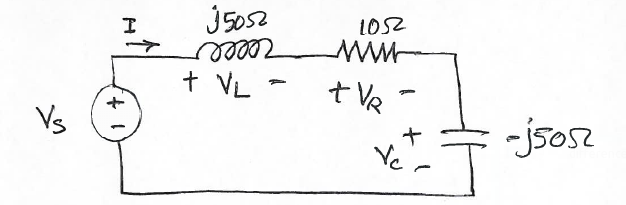
\includegraphics[width=0.8\textwidth]{samplecircuit.png}
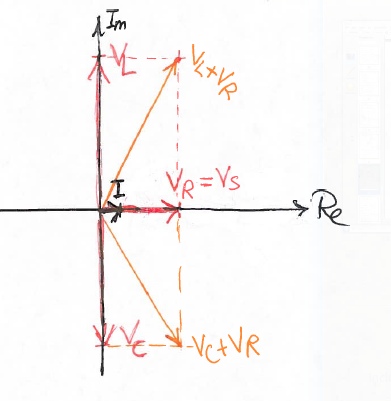
\includegraphics[width=0.5\textwidth]{samplecircuitsolved.png}
\end{figure}

\section*{AC Circuit Power Analysis}
In DC circuits, $v$, $i$, and $P = vi$ are constant with respect to time. For {\bf AC circuits}, these all are time varying. Thus, we have an instantaneous power which can be used to calculate average power.

\subsection*{Instantaneous Power}
When following the passive sign convention, we have $p(t) = v(t) * i(t)$

So for a resistor we have $p(t) = i^2(t)R$, for an inductor we have $p(t) = \frac{1}{L}\ v(t)\dint{-\infty}{t}{v(\tau)}{\tau}$ (assuming $v(-\infty) = 0$), and for a capacitor we have $p(t) = \frac{1}{C}\ i(t)\dint{-\infty}{t}{i(\tau)}{\tau}$ (assuming $v(-\infty) = 0$).

\subsection*{Average Power}
To find the {\bf average power} we have \[ P = \lim_{\tau\to\infty} \frac{1}{\tau} \dint{-\frac{\tau}{2}}{\frac{\tau}{2}}{p(t)}{t} \]

For periodic functions with period $T$, we can integrate over one period, or any integral number of periods $nT$ where $n in \mathbb{Z}$. Thus we have \[ P = \frac{1}{nT} \dint{t_0}{t_0+nT}{p(t)}{t} \]

For the sinusoidal case in steady state where $v(t) = V_m\cos(\omega t _ \theta)$ and $i(t) = I_m\cos(\omega t + \phi)$ we have \[ P = \frac{V_mI_m}{2}\cos(\theta - \phi) \]

\subsubsection*{Resistors}
Becase resistors are always in phase, we have \[ P = \frac{V_mI_m}{2} = \frac{1}{2}\frac{V_m^2}{R} = \frac{1}{2}I_m^2R \]

\subsubsection*{Purely Reactive Elements}
For inductors or capacitors, which are always $\frac{\pi}{2}$ out of phase, we have \[ P = 0 \]

This is because no power is absorbed by an ideal inductor or capacitor. FOr purely reactive networks, power flows in and out of the network with no power lost.

\newpage
\subsection*{Maximum Power Transfer}
For the following circuit
\begin{figure}[ht]
\centering
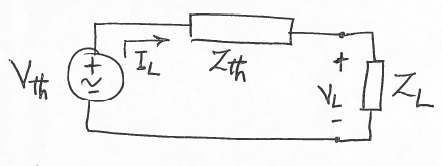
\includegraphics[width=0.5\textwidth]{impedance.png}
\end{figure}

to transfer the maximum amount of power, $Z_L = Z_{{\rm th}}^*$.

\subsection*{Effective Values of $I$ and $V$}
Definition: \textit{The effectiveness of any periodic current is equal to the value of the DC which, flowing through an R-ohm resistor, delivers the same average power to the resistor as does the periodic current.}

\[ I_{{\rm eff}} = I_{{\rm rms}} = \sqrt{\frac{1}{T}\dint{0}{T}{i^2(t)}{t}} \] and \[ V_{{\rm eff}} = V_{{\rm rms}} = \sqrt{\frac{1}{T}\dint{0}{T}{v^2(t)}{t}} \]

For sinusoidal values, we can simplify this as \[ I_{{\rm rms}} = \frac{I_m}{\sqrt{2}} \] and \[ V_{{\rm rms}} = \frac{V_m}{\sqrt{2}} \]

For the average power consumed by a resistor we have \[ P_R = \frac{V_mI_m}{2} = \frac{V_m}{\sqrt{2}}\frac{I_m}{\sqrt{2}} = V_{{\rm rms}}I_{{\rm rms}} \]

\subsection*{Apparent Power and the Power Factor}
The {\bf power factor} is the ratio of average power to apparent power, or \[ PF = \frac{P}{V_{{\rm rms}}I_{{\rm rms}}} = \cos(\theta - \phi) \]

For a purely resistive load, $PF = 1$. For a purely inductive or capacitive load, $PF = 0$. Thus we have $0 \leq PF \leq 1$.

Note that if we have $\theta - \phi > 0$, the current is lagging, thus we have an inductive load (and vice verse).

\subsection*{Complex Power}
For the average real power delivered to the network $P = {\rm Re}\{VI^*\}$ we may define the {\bf complex power} $S$ as \[ S = VI^* \] such that $|S| = V_{{\rm rms}}I_{{\rm rms}} =$ apparent power, and $\angle S = \theta - \phi =$ the power factor angle.

In rectangular form, we have $S = P + jQ$ where $P$ is the average power consumed by the network and $Q$ is the reactive power \[ Q = V_{{\rm rms}}I_{{\rm rms}}\sin(\theta - \phi) \]

Reactive power is the average rate of energy flow back and forth between the source and the reactive component of the load.
\end{document}
